% !TeX root = RJwrapper.tex
\title{A clustering algorithm to organize satellite hotspots data for the
purpose of tracking bushfires remotely}
\author{by Weihao Li, Emily Dodwell, and Dianne Cook}

\maketitle

\abstract{%
An abstract of less than 150 words.
}

\hypertarget{introduction}{%
\subsection{Introduction}\label{introduction}}

Bushfires are a major problem for Australia, and many other parts of the
globe. There is concern that as the climate becomes hotter, and drier,
that the impact of fires becomes much more severe and extensive. In
Australia, the 2019-2020 fires were the worst on record causing
extensive ecological damage, as well as damage to agricultural
resources, properties and infrastructure. The Wollemi pine, rare
prehistoric trees, required special forces intervention to prevent the
last stands in the world, in remote wilderness areas, from being turned
into ash.

Contributing to the problem is that many fires started in very remote
areas, locations deep into the temperate forests ignited by lightning,
that are virtually impossible to access or to monitor. Satellite data
provides a possible solution to this, particularly remotely sensed hot
spot data, which may be useful in detecting new ignitions and movements
of fires. Understanding fires in remote areas using satellite data may
provide some help in developing effective strategies for mitigating
bushfire impact.

This work addresses this topic. Using hot spot data, can we cluster in
space and time, in order to determine (1) points of ignition and (2)
track the movement of bush fires.

This paper is organised as follows. The next section provides an
introduction to the literature on spatiotemporal clustering and bush
fire modeling and dynamics. Section
\protect\hyperlink{algorithm}{Algorithm} describes the clustering
algorithm, and section \protect\hyperlink{application}{Application}
illustrates how the resulting data can be used to study bush fire
ignition.

\hypertarget{background}{%
\subsection{Background}\label{background}}

\hypertarget{spatiotemporal-clustering}{%
\subsubsection{Spatiotemporal
clustering}\label{spatiotemporal-clustering}}

\hypertarget{bushfire-modeling}{%
\subsubsection{Bushfire modeling}\label{bushfire-modeling}}

\hypertarget{algorithm}{%
\subsection{Algorithm}\label{algorithm}}

\hypertarget{data-pre-processing}{%
\subsubsection{Data pre-processing}\label{data-pre-processing}}

\begin{Schunk}
\begin{figure}
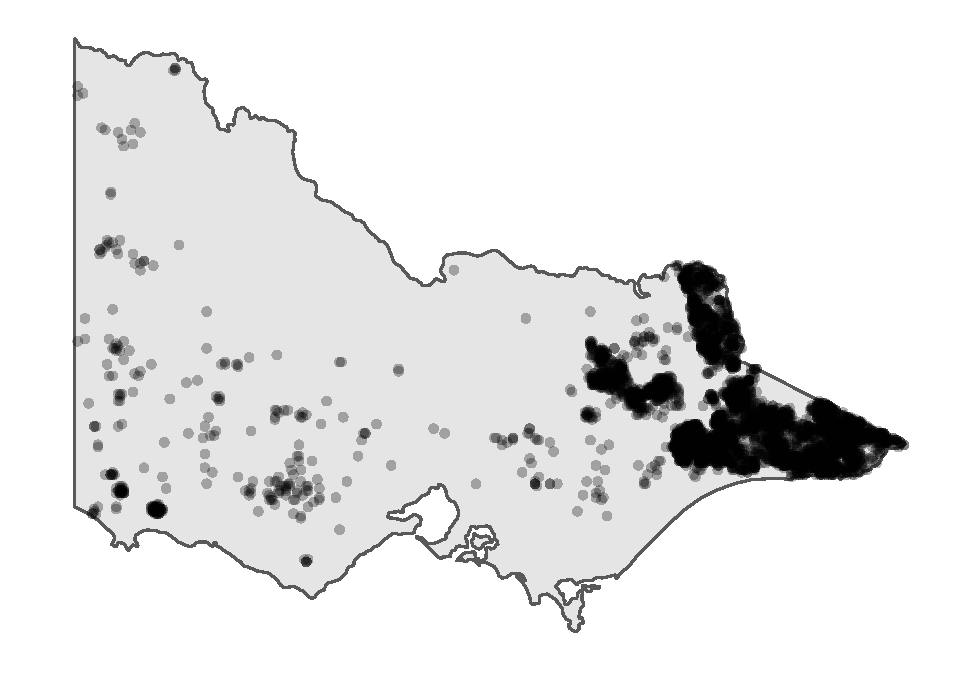
\includegraphics[width=0.8\linewidth]{clustering_paper_files/figure-latex/hotspots-1} \caption[Hotspot locations in Victoria during 2019-2020 season]{Hotspot locations in Victoria during 2019-2020 season.}\label{fig:hotspots}
\end{figure}
\end{Schunk}

\hypertarget{steps}{%
\subsubsection{Steps}\label{steps}}

This algorithm runs in a temporal manner. Starting from the first hour
of the first day or the bushfire season, hotspots are grouped, and then
agglomerated spatially. This proceeds to the next hour.

\textbf{1. Divide hotspots by hour}

The algorithm starts by dividing hotspots into subgroups given their
hours since the first observed hotspot as shown in Figure
\ref{fig:step1}. Notice the unit of time is an arbitrary choice.
Theoretically, it can be replaced with any other units not larger than
the total length of time and not less than the temporal resolution of
the data. Normally, the algorithm will be sensitive to noises and
unobserved hotspots if a small unit of time is used while losing details
of bushfires movement if a large unit of time is used.

One hour is chosen to be the default unit of time because the temporal
resolution of our data is 10 minutes. Besides, since bushfires usually
last longer than 12 hours, treating hotspots within an hour as a whole
is reasonable.

\begin{Schunk}
\begin{figure}
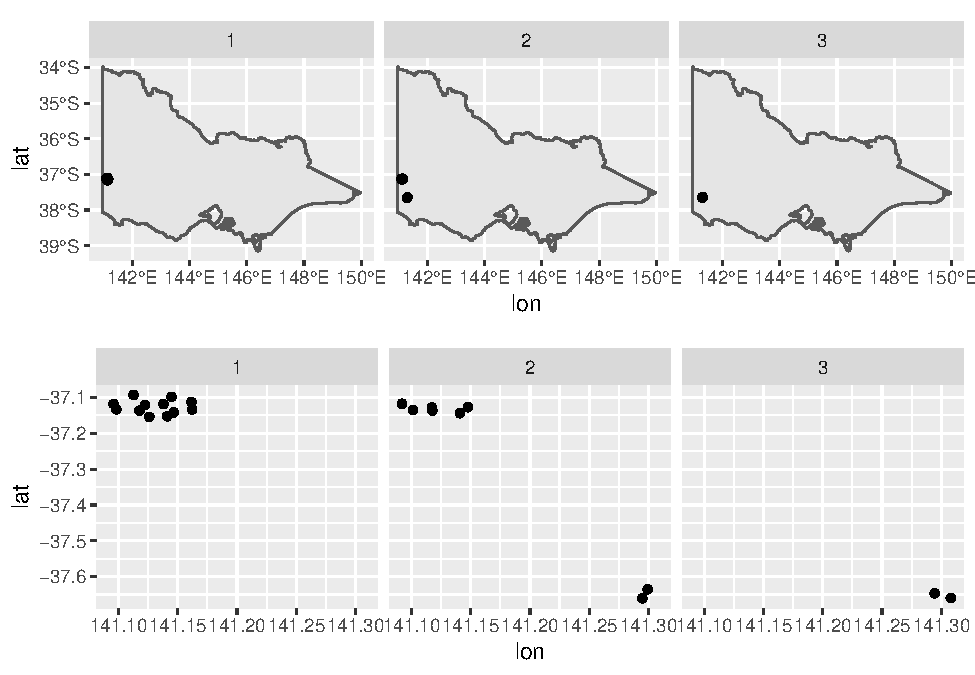
\includegraphics[width=0.8\linewidth]{clustering_paper_files/figure-latex/step1-1} \caption[Step 1]{Step 1. Hotspots in the first 3 hours of the bushfire season.}\label{fig:step1}
\end{figure}
\end{Schunk}

\textbf{2. Start from the first hour}

The algorithm first selecting the hotspots in the first hour as shown in
Figure \ref{fig:step2}.

\begin{Schunk}
\begin{figure}
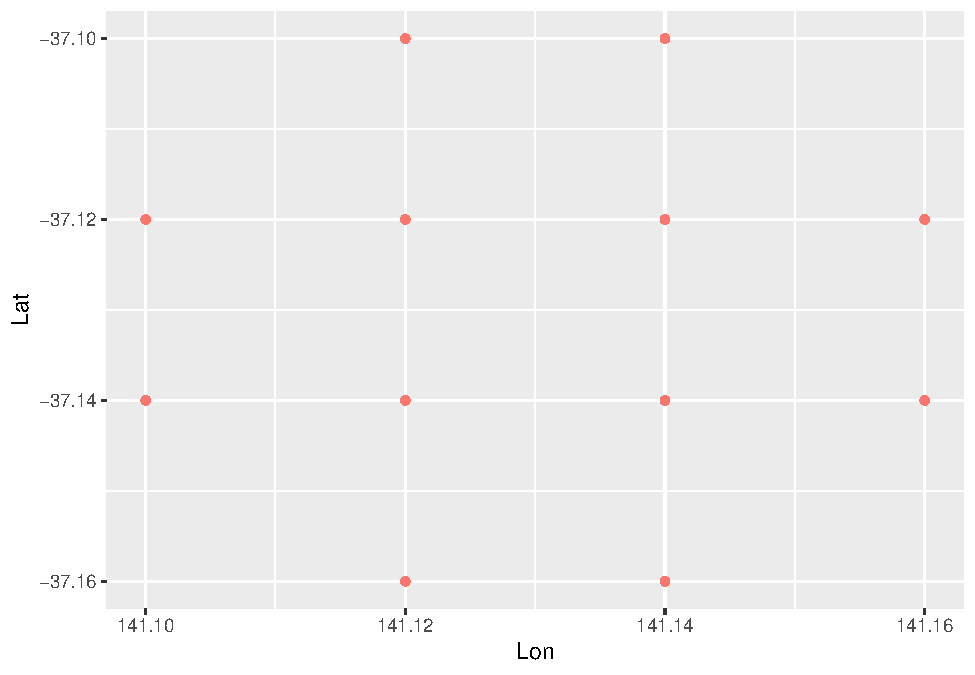
\includegraphics[width=0.8\linewidth]{clustering_paper_files/figure-latex/step2-1} \caption[Step 2]{Step 2. Hotspots in the first hour.}\label{fig:step2}
\end{figure}
\end{Schunk}

\textbf{3. Connect reachable hotspots}

We try to formalize the meaning of ``cluster'' to better illustrate the
connection between this algorithm and the underlying bushfire behaviour.
When bushfires spread over time, the satellite will record a series of
hotspots along its trajectory. Thus, if two hotspots are close to each
other within a certain distance in a short period of time, they could be
considered as a single bushfire.

\begin{defn}[directly reachable] A point p is directly reachable from a point q with respect to AdjDist, if the distance between point p and q is less or equal to AdjDist.\end{defn}

\begin{defn}[reachable] A point p is reachable from a point q with respect to AdjDist, if there is a chain of points $p_1$, $p_2$, ..., $p_n$, $p_1 = p$, $P_n = q$ such that $P_n$ is directly reachable from $p_{n-1}$. \end{defn}

In this step, the algorithm connects all pairs of directly reachable
hotspots with respect to \(AdjDist = 3000m\) in the first hour as shown
in Figure \ref{fig:step3}. The result of this step is an undirected and
unweighted graph. \(AdjDist\) is the first parameter used in this
algorithm which controls the connectivity between hotspots. It is
introduced for the purpose of parameterizing the speed of bushfires.

\begin{Schunk}
\begin{figure}
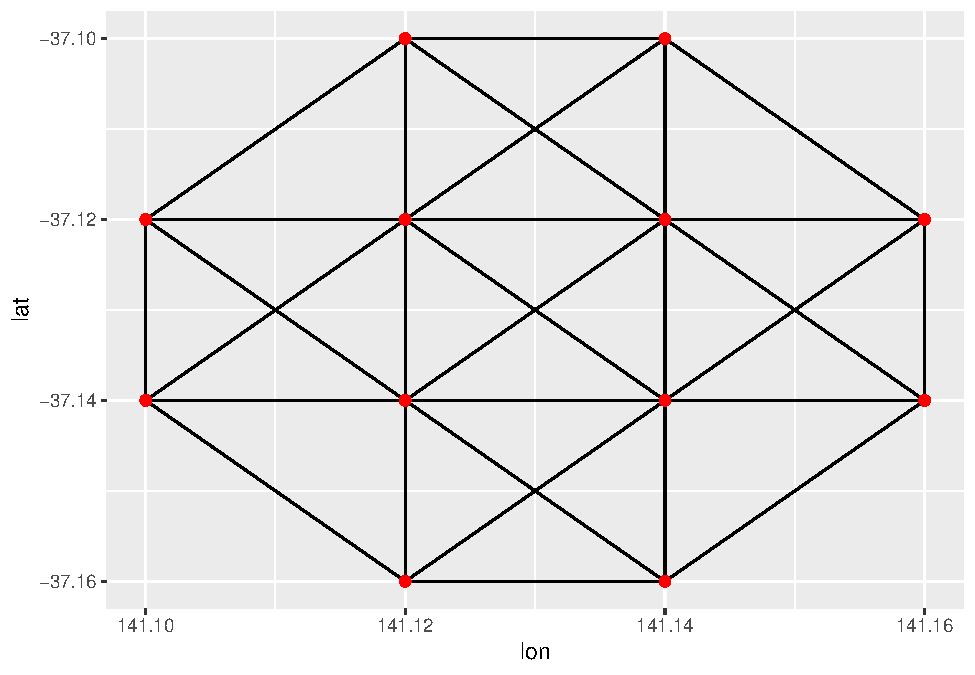
\includegraphics[width=0.8\linewidth]{clustering_paper_files/figure-latex/step3-1} \caption[Step 3]{Step 3. All pairs of directly reachable hotspots in the first hour are connected given the AdjDist is 3000 metres. There is only one component in the graph}\label{fig:step3}
\end{figure}
\end{Schunk}

\textbf{4. Assign memberships to hotspots}

The algorithm then clusters hotspots into groups based on the
connectivity between hotspots as shown in Figure \ref{fig:step4}.
Different memberships will be assigned to vertices in different
components. Thus, if two hotspots are reachable from each other, they
will be assigned the same membership. In the first hour, because all
hotspots are reachable from other hotspots, they are assigned the same
membership.

\begin{Schunk}
\begin{figure}
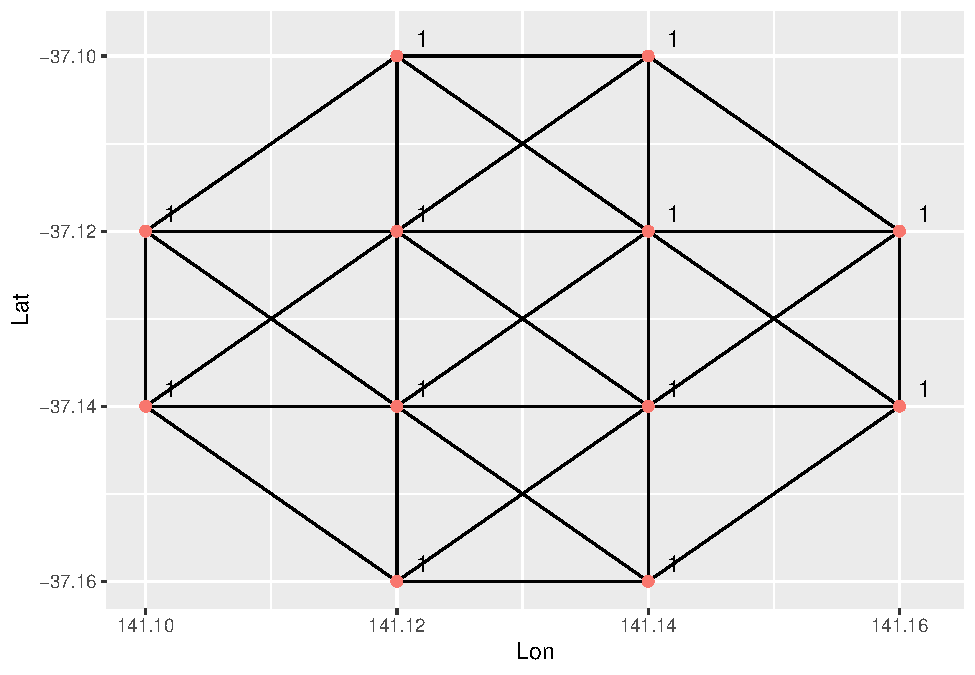
\includegraphics[width=0.8\linewidth]{clustering_paper_files/figure-latex/step4-1} \caption[Step 4]{Step 4. All hotspots in the first hour are reachable from each other. They are assigned the same membership.}\label{fig:step4}
\end{figure}
\end{Schunk}

\textbf{5. Move to the second hour or beyond}

We need to introduce the second parameter used in this algorithm, which
is ActiveTime. This parameter controls the time frame of hotspots that
will be included by the algorithm in each iteration. More specifically,
this time frame is defined as \([max(t-ActiveTime,1),t]\), where \(t\)
is the current timestamp of the algorithm. For instance, if
\(ActiveTime = 24\) and the algorithm is clustering the hotspots in the
36th hour, then the time frame will be \([12,36]\).

We define this time frame for the purpose of associating the hotspots in
the current timestamp with hotspots observed in previous hours. By
imposing this time frame, we provide an invariant task at each
iteration, which is clustering hotspots in the current hour given the
clustered hotspots in previous hours.

Move to the hour \(t\), the algorithm will select hotspots in hour
between \(max(t-ActiveTime,1)\) and \(t\), including
\(max(t-ActiveTime,1)\) and \(t\). Given \(t = 2\) and
\(ActiveTime = 24\), the hotspots in the first two hours will be
selected as shown in Figure \ref{fig:step5}.

\begin{Schunk}
\begin{figure}
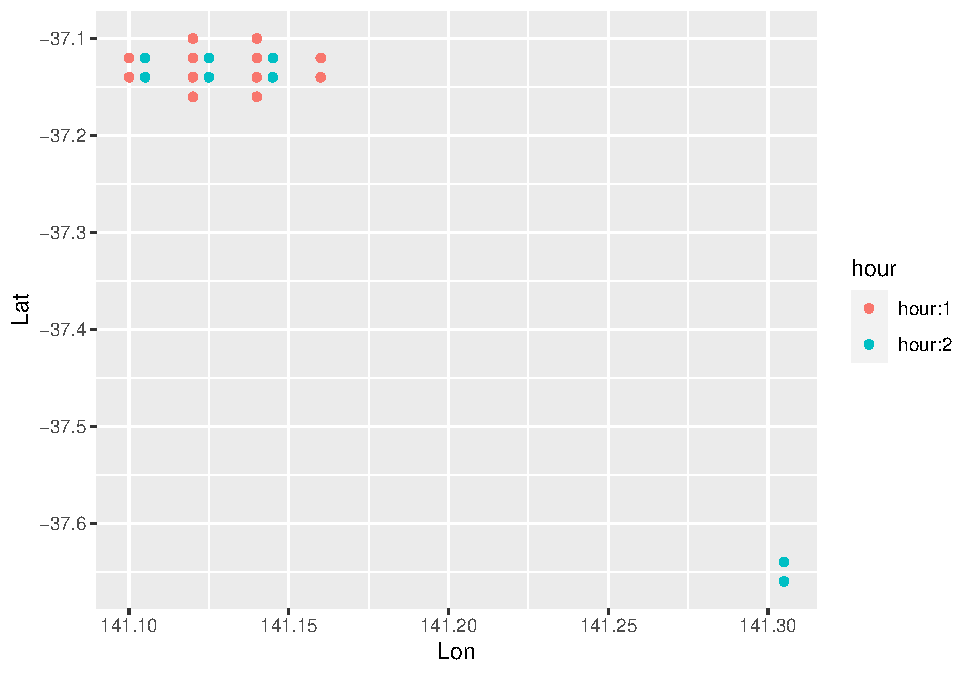
\includegraphics[width=0.8\linewidth]{clustering_paper_files/figure-latex/step5-1} \caption[Step 5]{Step 5. Hotspots in the first two hours. Due to overlapping, hotspots in the second hour are adjusted by 0.005 degree in longitude.}\label{fig:step5}
\end{figure}
\end{Schunk}

\textbf{6. Connect reachable hotspots}

This step is equivalent to step 3 and is only used for illustration
purpose. Given the hotspots in the first two hours, the algorithm
connects all pairs of reachable points as shown in Figure
\ref{fig:step6}.

\begin{Schunk}
\begin{figure}
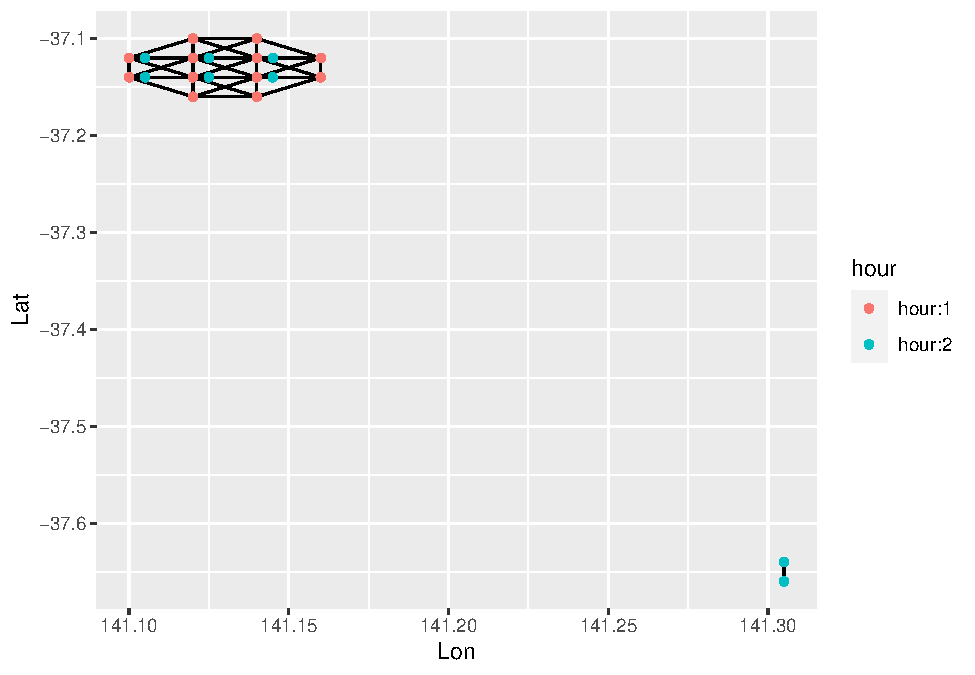
\includegraphics[width=0.8\linewidth]{clustering_paper_files/figure-latex/step6-1} \caption[Step 6]{Step 6. All pairs of directly reachable hotspots in the first two hours are connected given the AdjDist is 3000 metres. There are two components in the graph.}\label{fig:step6}
\end{figure}
\end{Schunk}

\textbf{7. Find the nearest hotspot in the previous hours within the
same component for each hotspots in the current timestamp}

According to the result from step 6, the algorithm will then find the
nearest hotspot in the previous hours within the same component for each
hotspots in the current timestamp which is the second hour as shown in
Figure \ref{fig:step7}. This step along with step 8 is to solve the
problem when a hotspot in the current timestamp share the same component
with multiple hotspots in the previous hours. And, we need to decide
which membership in the previous hours it should inherit.

\begin{Schunk}
\begin{figure}
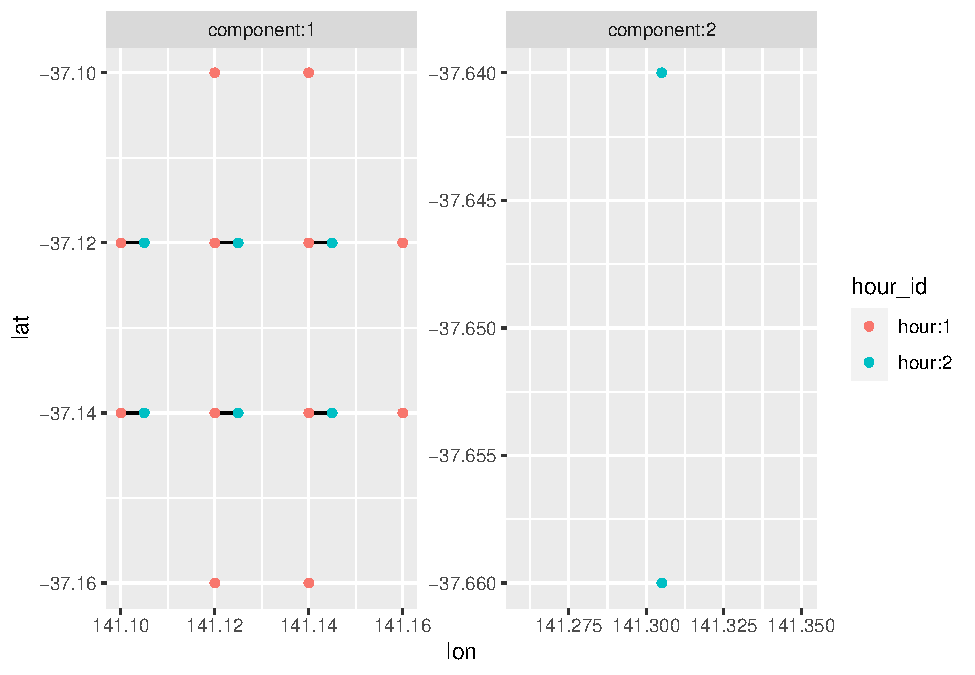
\includegraphics[width=0.8\linewidth]{clustering_paper_files/figure-latex/step7-1} \caption[Step 7]{Step 7. Hotspots in the second hour is connected with its nearest hotspot in the first hour within the same component. Due to overlapping, hotspots in the second hour are adjusted by 0.005 degree in longitude.}\label{fig:step7}
\end{figure}
\end{Schunk}

\textbf{8: Assign membership to hotspots in the current timestamp}

\hypertarget{effects-of-parameter-choices}{%
\subsubsection{Effects of parameter
choices}\label{effects-of-parameter-choices}}

There are two parameters that can be tuned in this algorithm. They are
\texttt{adj\_dist}, which is the density distance and
\texttt{active\_time}, which is the .

\hypertarget{application}{%
\subsection{Application}\label{application}}

\hypertarget{determining-the-ignition-point-and-time-for-individual-fires}{%
\subsubsection{Determining the ignition point and time for individual
fires}\label{determining-the-ignition-point-and-time-for-individual-fires}}

Show ignition points for a particularly heavy day and another for a
particularly light day

\begin{Schunk}

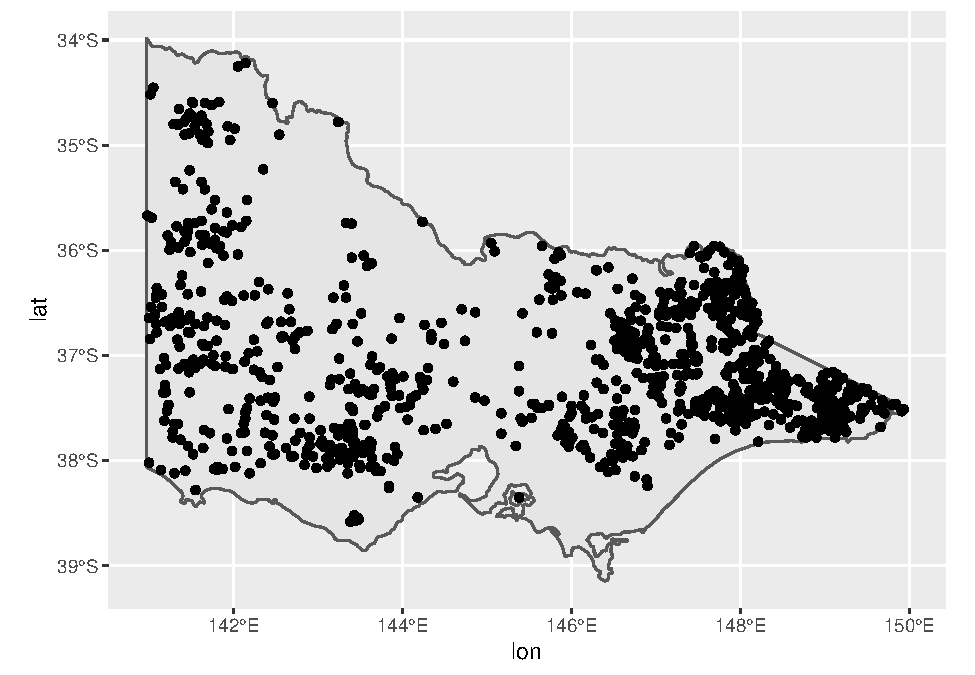
\includegraphics[width=0.8\linewidth]{clustering_paper_files/figure-latex/unnamed-chunk-2-1} \end{Schunk}

\begin{Schunk}

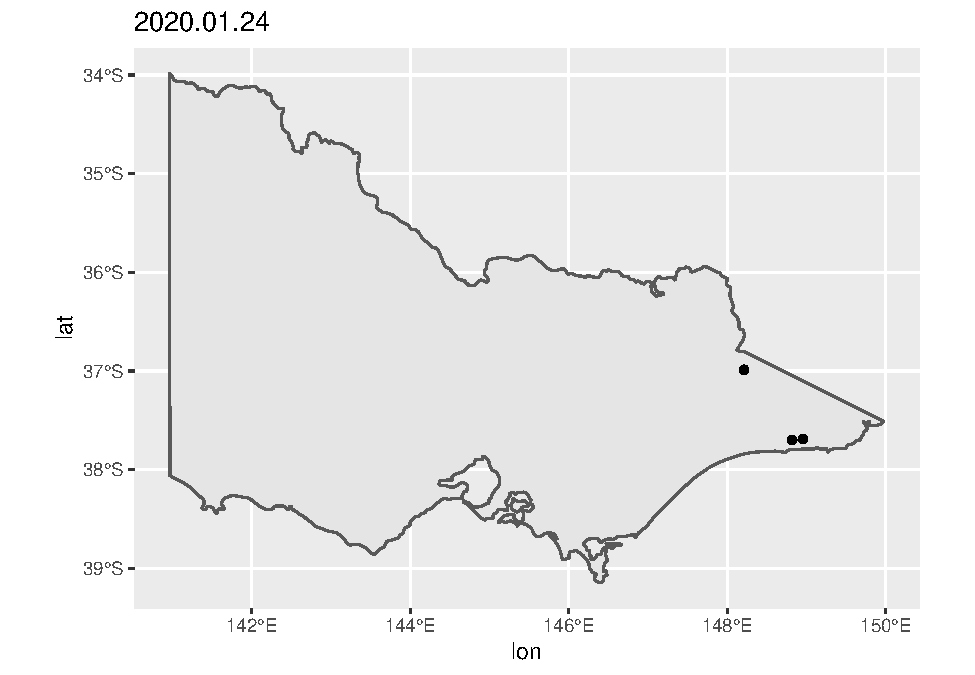
\includegraphics[width=0.8\linewidth]{clustering_paper_files/figure-latex/unnamed-chunk-4-1} \end{Schunk}

\begin{Schunk}

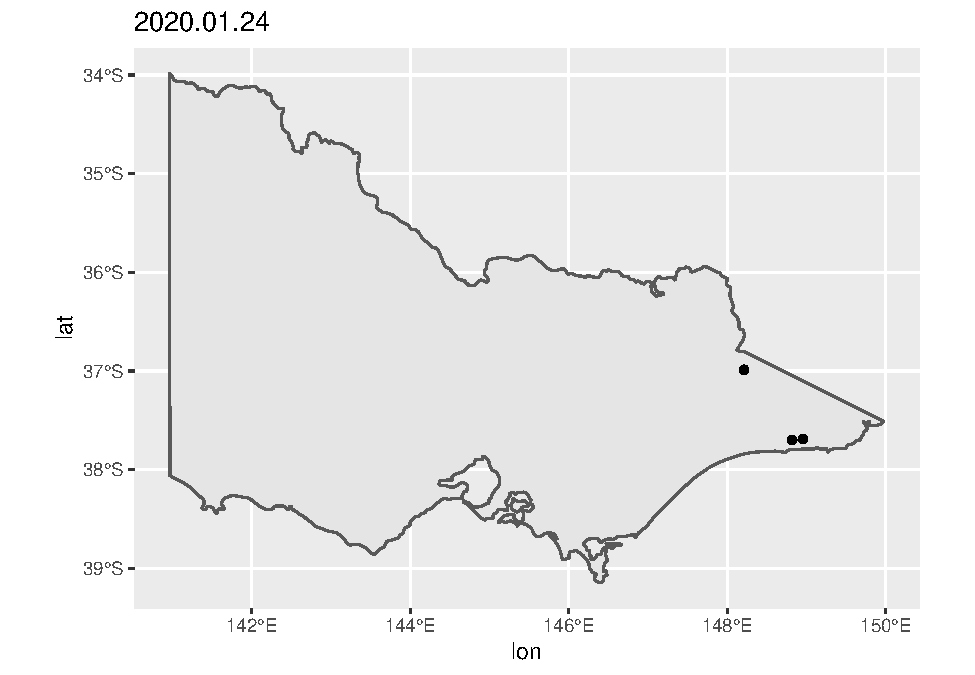
\includegraphics[width=0.8\linewidth]{clustering_paper_files/figure-latex/unnamed-chunk-5-1} \end{Schunk}

\hypertarget{tracking-fire-movement}{%
\subsubsection{Tracking fire movement}\label{tracking-fire-movement}}

Display showing how a fire moves over time, maybe two or more fires

\hypertarget{allocating-resources-for-future-fire-prevention}{%
\subsubsection{Allocating resources for future fire
prevention}\label{allocating-resources-for-future-fire-prevention}}

Merging data with camp sites, CFA, roads, \ldots{}

\hypertarget{summary}{%
\subsection{Summary}\label{summary}}

\hypertarget{acknowledgements}{%
\subsection{Acknowledgements}\label{acknowledgements}}

\begin{itemize}
\tightlist
\item
  The code and files to reproduce this work are at XXX
\item
  Data on hotspots can be downloaded from XXX
\end{itemize}

\bibliography{RJreferences}


\address{%
Weihao Li\\
Monash University\\%
line 1\\ line 2\\
%
%
%
\\\href{mailto:wlii0039@student.monash.edu}{\nolinkurl{wlii0039@student.monash.edu}}
}

\address{%
Emily Dodwell\\
AT\&T\\%
line 1\\ line 2\\
%
%
%
\\\href{mailto:emily@research.att.com}{\nolinkurl{emily@research.att.com}}
}

\address{%
Dianne Cook\\
Monash University\\%
line 1\\ line 2\\
%
%
%
\\\href{mailto:dicook@monash.edu}{\nolinkurl{dicook@monash.edu}}
}

